\documentclass{article}

\usepackage[utf8]{inputenc}
\usepackage[T1]{fontenc}
\usepackage{lipsum}
\usepackage{graphicx}
\usepackage{amsmath}
\usepackage[margin=1in]{geometry}
\usepackage{titlesec}
\usepackage{graphicx}
\usepackage{floatflt,epsfig}
\usepackage[utf8]{inputenc}
\usepackage[T1]{fontenc}
\usepackage{tabularx}
\usepackage{lipsum}
\usepackage{graphicx}
\usepackage{amsmath}
\usepackage[margin=1in]{geometry} 
\usepackage{titlesec}
\usepackage{listings}
\usepackage{xcolor}

\lstdefinelanguage{XML}
{
  morestring=[b]",
  morestring=[s]{>}{<},
  morecomment=[s]{<?}{?>},
  morecomment=[s][\color{green!50!black}]{<!--}{-->},
  stringstyle=\color{blue},
  identifierstyle=\color{red},
  keywordstyle=\color{orange},
  commentstyle=\color{green!50!black},
  basicstyle=\small\ttfamily,
  frame=single, 
  breaklines=true,
  breakatwhitespace=true,
  tabsize=2,
  showstringspaces=false,
  captionpos=b,
}

\lstdefinelanguage{Java}{
  keywords={abstract,assert,boolean,break,byte,case,catch,char,class,const,continue,default,do,double,else,enum,extends,false,final,finally,float,for,goto,if,implements,import,instanceof,int,interface,long,native,new,null,package,private,protected,public,return,short,static,strictfp,super,switch,synchronized,this,throw,throws,transient,true,try,void,volatile,while},
  morekeywords={[2]System,out},
  morecomment=[l]{//},
  morecomment=[s]{/*}{*/},
  morestring=[b]",
  basicstyle=\small\ttfamily,
  keywordstyle=\color{blue}\bfseries,
  keywordstyle={[2]\color{orange}\bfseries},
  commentstyle=\color{green!70!black},
  stringstyle=\color{red},
  showstringspaces=false,
  tabsize=2,
  breaklines=true,
  breakatwhitespace=true,
  frame=single, 
  captionpos=b
}


\titleformat{\section}
{\LARGE\bfseries}{\thesection}{1em}{}

\titleformat{\subsection}
{\Large\bfseries}{\thesection}{1em}{}

\begin{document}

\pagestyle{empty}

\section*{Resources}
\large
Android è progettato per essere eseguito su un innumerevole insieme di dispositivi. In questo ambito ogni applicazione sviluppata dovrebbe attuare \textit{feature} dinamiche, rendendo adattiva la \textit{user interface} rispetto alle configurazioni dello schermo.\vspace*{14pt}\\
Come già accennato un'applicazione Android dovrebbe essere eseguita su una eterogenità di dispositivi, ognuno di essi con le proprie caratteristiche. Per riuscire nell'intento possono essere adeguati due approcci principali:
\begin{enumerate}
    \itemsep0em
    \renewcommand*{\labelenumi}{-}
    \item \textbf{Soluzione tradizionale}, adottare tutte le molteplici alternative. Tuttavia questo si traduce in un abuso di costrutti condizionali, rendendo il codice di difficile lettura; inoltre occorre ricompilare il progetto ogni qualvolta dovesse presentarsi la necessità di variare il \textit{Layout} oppure qualora aggiunti nuovi \textit{package}
    \item \textbf{Soluzione Android}, separare il codice dalle \textit{risorse}. Rispetto al paradigma descritto si usufruisce dell'approccio dichiarativo XML affinchè possano essere definite le risorse
\end{enumerate}
Prima di addentrarsi all'interno della composizione delle cartelle che caratterizzino un progetto è bene stabilire cosa sia una \textit{risorsa}.\vspace*{7pt}\\
\textit{Definizione}\\
Una \textit{risorsa} è tutto ciò che non sia codice.\vspace*{7pt}\\
Pur di rispettare la definizione precedente è necessario che si susseguano tre condizioni:
\begin{enumerate}
    \itemsep0em
    \renewcommand*{\labelenumi}{-}
    \item Separare gli aspetti visivi dagli aspetti gestionali. In tal senso si prosegue mediante il paradigma di "buon codice", ossia separare ciò che possa essere ritenuto associabile alla \textit{business logic} da ciò che contraddistingue la \textit{user interface}
    \item Provvedere a garantire un numero elevato di \textit{features} che possano coprire il più ampio insieme di dispositivi
    \item Ricompilare solamente quando strettamente necessario
\end{enumerate}
Solitamente è preferita la soluzione Android, data soprattutto dalla capacità del framework di rilevare tutte le caratteristiche configurative del dispositivo, associandone la risorse appropiate, e dalla facilità con cui sia possibile aggiungere nuove resources per supportare un'ulteriore categoria di device.\vspace*{14pt}\\
All'interno di un qualsiasi progetto le risorse sono destinate all'interno della directory \textbf{res}; si tratta di una gerarchia già predisposta per i molteplici package inseriti.

\subsection*{Resources Definition}
Le risorse sono inizializzate mediante il metodo \textbf{dichiarativo} espresso dai file \textbf{XML}, in cui ognuna di esse possiede un proprio nome e identificativo.\vspace*{7pt}
\begin{lstlisting}[language=XML, title=Dichiarazione delle risorse mediante file XML]
<resources> 
    <string name="hello">Hello World!</string>
    <string name="labelButton">Insert your name</string>
</resources>
\end{lstlisting}
Tali risorse possono essere acquisite tramite la \textbf{classe R}, il cui funzionamento simula un \textit{collante} tra il codice e il documento XML; si tratta di un file generato e gestito automaticamente, ricreato qualora dovessero essere riportate delle modifiche.\vspace*{7pt}\\
Applica il design pattern \textit{Singleton}, pertanto l'intero progetto sviluppato fonda sulla singola istanza della classe. Quindi, ricapitolando, \textbf{R} contiene tutti gli identificativi delle resources poste all'interno della directory \textit{res}.\vspace*{7pt}
\begin{lstlisting}[language=JAVA, title=Definizione della classe R]
public finale class R {
    public static final class string {
        public static final int hello=0x7040001;
        public static final int labelButton=0x7040005;
    }    
}
\end{lstlisting}
L'\textit{ID} definito precedentemente è composto da due sezioni esplicative, definite come segue:
\begin{enumerate}
    \itemsep0em
    \renewcommand*{\labelenumi}{-}
    \item Il \textbf{type}, ossia il tipo della risorsa, ad esempio string, menu, layout ...
    \item Il \textbf{name}, a sua volta contraddistinto dal \textit{filename} e dal \textit{value} posto all'interno del documento XML 
\end{enumerate}
Proseguendo, esistono due modalità di accesso al contenuto delle risorse:
\begin{enumerate}
    \itemsep0em
    \renewcommand*{\labelenumi}{-}
    \item Accesso tramite XML, in cui è attuata una sintassi simile a
    \begin{center}
        \textit{@[<package\_name>:]<resource\_type>/<resource\_name>}
    \end{center}
    Il \textit{@[<package\_name>:]}, oltre ad essere una sezione opzionale, definisce il nome del \textit{package} in cui la risorsa è allocata. Il \textit{<resource\_type>} è il nome del \textit{tipo} della risorsa. Il \textit{<resource\_name>} rappresenta il \textit{filename} della risorsa.\vspace*{7pt}\\
    Di seguito è proposto un titolo esemplificativo, in maniera tale che possa essere definito nel migliore dei modi il concetto espresso prima.
    \begin{lstlisting}[language=XML, title=Accesso al contenuto delle risorse mediante XML]
<LinearLayout>
    <TextView android:id="@+id/label1"
        android:text="@string/labelText" android:textcolor="@android:color/black"/>
    <Button android:id="@+id/button1" android:text="@string/labelButton"
        android:background="@color/my_red"/>
</LinearLayout>
    \end{lstlisting}
    Da esempio sono differenti i punti salienti in cui occorre soffermarsi. Nella dichiarazione della \textit{TextView} si nota l'utilizzo della sintassi \textit{<resource\_type>/<resource\_name>}, definita in \textit{android:text="@string/labelText"}, mentre, sempre nella medesima sezione, si evidenzia la presenza di un value in cui è espresso il \textit{@[<package\_name>:]}, in \textit{android:textcolor="@android:color/black"}. Contrariamente, all'interno del tag \textit{Button} è visualizzata la denominazione di un ulteriore \textit{package name}, in questo case ritrae un pacchetto ideato dallo sviluppatore e non dato built-in da Android, come da nomenclatura precedente.
    \item Accesso tramite \textit{codice Java/Kotlin}, dove la sintassi adeguata promuove
    \begin{center}
        \textit{[package\_name]R.resource\_type.resource\_name}
    \end{center}
    Nuovamente, il \textit{package\_name} definisce il \textit{package} in cui la risorsa è allocata. Il \textit{resource\_type} è il nome del \textit{tipo} della risorsa. Il \textit{resource\_name} è la denominazione del \textit{filename}.\\
    \begin{lstlisting}[language=JAVA, title=Accesso al contenuto delle risorse mediante Kotlin]
val hello:String = this.getResource().getString(R.string.hello)
val myRed:Color = getResource().getString(R.color.my_red)
val msgTextView = findViewById(R.id.label1) as TextView
msgTextView.setText(R.string.labelText)
    \end{lstlisting}    
In relazione allo sketch di codice proposto, possono essere evidenziate alcuna peculiarità. Alla variabile \textit{hello} è assegnata una stringa contenuta all'interno del file \textit{string.xml}; l'accesso è definito esattamente come stabilito dalla sintassi precedente, in cui è dichiarata la classe \textit{R}, il \textit{tipo} ed infine il \textit{nome} della risorsa. Si sottolinea come in questa casistica affinchè possa essere garantito l'assegnamento, occorre stabilire preventivamente il \textit{contesto} e la \textit{funzione} che ne permettano il corretto svolgimento, espresso come \textit{context.getResource()}; contrariamente in casi in cui non sia necessario allocare il contesto può essere omesso.
\end{enumerate}\vspace*{7pt}
La sezione successiva definisce come utilizzare tipi e strutture dati, in maniera tale che sia fornita una prima panoramica.

\subsection*{Values}
\begin{center}
    \begin{lstlisting}[language=XML, title=Manipolazione di tipi primitivi e strutture dati in XML]
<resources>
    <string name="label">Example application</string>
    <integer name="value">58</integer>
    <string-array name="nameArray">
        <item>Ciao</item>
        <item>Hello</item>
        <item>Hola</item>
    </string-array>
    <integer-array name="valArray">
        <item>1</item>
        <item>2</item>
        <item>3</item>
    </integer-array>
</resources>
    \end{lstlisting}  
\end{center}
\begin{center}
    \begin{lstlisting}[language=JAVA, title=Manipolazione di tipi primitivi e strutture dati in Kotlin]
val label:String = resources.getString(R.string.label)
val value:Int = resources.getInteger(R.integer.value)
val nameArray:Array<Integer> = resources.getStringArray(R.array.nameArray)
val valArray:Array<Integer> = resources.getIntegerArray(R.array.valArray)
    \end{lstlisting}  
\end{center}
\begin{center}
    \begin{lstlisting}[language=XML, title=Manipolazione di risorse color in XML]
<resources>
    <color name="coin_yellow">#FF9800</color>
    <color name="coin_yellow">#FF3131</color>
</resources>
    \end{lstlisting}  
\end{center}
\begin{center}
    \begin{lstlisting}[language=JAVA, title=Manipolazione di risorse color in Kotlin]
val coinColor:Int = resources.getColor(R.color.coin_yellow, null)
    \end{lstlisting}  
\end{center}
\begin{center}
    \begin{lstlisting}[language=XML, title=Manipolazione di risorse dimension in XML]
<resources>
    <dimen name="textview_height">25dp</dimen>
    <dimen name="textview_width">150dp</dimen>
    <dimen name="font_size">20sp</dimen>
</resources>
    \end{lstlisting}  
\end{center}
\begin{center}
    \begin{lstlisting}[language=XML, title=Assegnamento delle dimen agli attributi del XMl layout]
<TextView
    android:layout_height="@dimen/textview_height"
    android:layout_width="@dimen/textview_width"
    android:textSize="@dimen/font_size"/>
    \end{lstlisting}  
\end{center}
Uno \textbf{style} è un insieme di attributi, che possono essere applicati ad uno specifico elemento grafico della \textit{GUI} oppure ad intere schermate dell'applicazione. Generalmente si tratta di un file XML, referenziato mediante l'utilizzo dell'identificativo riportato all'interno dell'attributo designato.\vspace*{7pt}\\
Un'ulteriore peculiarità prevede la possibilità di attuare il paradigma di \textit{inheritance}, ossia organizzare gli stili mediante una gerarchia, dove ognuno di essi può acquisire proprietà grafiche da \textit{style} corrispondenti. La sintassi adottata per la dichiarazione di uno stile prevede l'uso dei seguenti tag \textit{<style>...</style>}, tipicamente creato all'interno della directory \textit{/res}.
\begin{lstlisting}[language=XML, title=Dichiarazione di uno style]
<resources>
    <style name="MyTheme" parent="Theme.Material3.DayNight.NoActionBar">
        <item name="colorPrimary">@color/coin_yellow</item>
        <item name="colorSecondary">@color/hound_grey</item>
    </style>
</resources>
\end{lstlisting}  
\begin{lstlisting}[language=XML, title=Assegnamento dello stile ad un solo elemento grafico]
<Button style="@style/MyTheme"
    android:layout_width="0dp"
    android:layout_height="wrap_content"
    android:text="Push me!" />    
\end{lstlisting}  
\begin{lstlisting}[language=XML, title=Assegnamento dello stile all'intera applicazione]
<application
    ...
    android:theme="@style/MyTheme"
>...</ application>    
\end{lstlisting}  
Gli sketch di codice definiti precedentemente testimoniano la volontà di realizzare applicazione legate alla scrittura di "buon" codice, non solo a livello di operatività, ma anche sotto l'aspetto archittetturale delle molteplici directories, in cui si evidenzia come ogni componente abbia la sua locazione apposita, dove lo strumento degli identificativi ne facilita l'accesso.

\subsection*{Resource Alternatives}
Le applicazioni \textit{Android} dovrebbero provvedere a risorse alternative in base alla tipologia e configurazione del device di riferimento. Durante \textit{runtime} Android rileva le caratteristiche correnti del dispositivo e carica le \textit{resources} appropriate per l'applicazione.\vspace*{7pt}\\
Per definire appropiatamente le \textit{resource alternatives} occorre attuare due step fondamentali:
\begin{enumerate}
    \itemsep0em
    \renewcommand{\labelenumi}{-}
    \item Creare una nuova \textit{directory} all'interno di \textit{/res}, denominata \textit{<resource\_name>-<qualifier>}
    \item Salvare la \textit{risorsa alternativa} all'interno della cartella
\end{enumerate}
Di seguito è proposto il principio di funzionameno secondo cui Android riesce a descriminare quali risorse siano associabili alla configurazione del dispositivo. Quando l'applicazione richiede una risorsa, Android seleziona l'\textit{alternative resource} da attuare durante \textit{runtime}, tramite l'algoritmo mostrato in figura. 
\begin{center}
    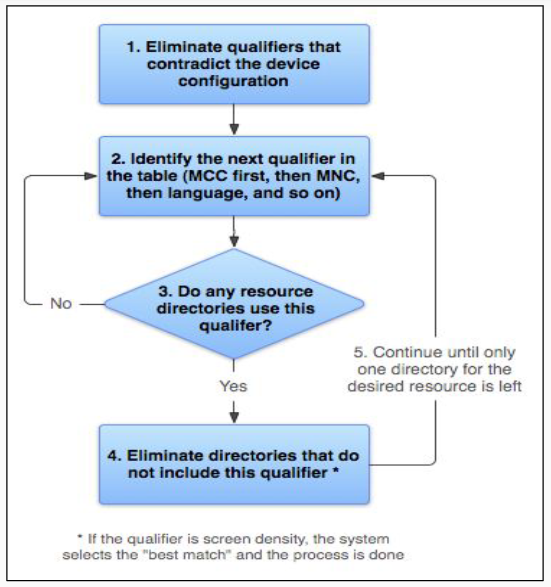
\includegraphics[width=0.5\textwidth]{foto1.png}
\end{center}
Come da algoritmo si notano cinque azioni principali, suddivise in:
\begin{enumerate}
    \itemsep0em
    \renewcommand{\labelenumi}{-}
    \item \textit{Step 1}, eliminare tutti i \textit{qualifiers} che contraddicono la configurazione del dispositivo
    \item \textit{Step 2}, identificare il prossimo \textit{qualifier} all'interno della tabella
    \item \textit{Step 3}, stabilire se qualsiasi cartella presente all'interno di \textit{resource} utilizzi il \textit{qualifier} giudicato
    \item \textit{Step 4a}, eliminare tutte le \textit{directories} che non includono il \textit{qualifier}
    \item \textit{Step 4b}, il processo continua fino a quando non sia rimasta una singola cartella 
\end{enumerate}
Ricapitolando elimina tutti i \textit{qualifiers} che contraddicono le specifiche del device.
\end{document}